%This is a experiment example of ZhengXiaoyang's experiment report template

\documentclass[UTF8]{ctexart}
 
\usepackage{pythonhighlight}
\usepackage{amsmath}
\usepackage{cases}
\usepackage{cite}
\usepackage{xeCJK}
\usepackage{graphicx}
\usepackage[margin=1in]{geometry}
\geometry{a4paper}
\usepackage{fancyhdr}
\pagestyle{fancy}
\fancyhf{}

\graphicspath{{picture/}}


\title{利用分光计测量玻璃的色散曲线实验报告}
\graphicspath{{picture/}}


\title{利用分光计测量玻璃的色散曲线实验报告}
\author{郑晓旸}
\date{\today}
\pagenumbering{arabic}

\begin{document}
%这里是文件的开头
\fancyhead[L]{郑晓旸}
\fancyhead[C]{色散曲线}
\fancyfoot[C]{\thepage}

\maketitle
\newpage
\tableofcontents
\newpage

\section{实验目的}
    \begin{enumerate}
            \item 掌握分光计的调整方法;
            \item 掌握利用最小偏向法测量三棱镜折射率的方法。
    \end{enumerate} 


\section{实验仪器}
\begin{enumerate}
    \item 分光计
    \item 低压汞灯
    \item 三棱镜
    \item 双面平面镜
    \item 其他辅助器件
\end{enumerate}

\section{实验原理}
\subsection{光的色散}
\subsubsection{介质中的光速}
与真空中光速不同,介质中光速对于不同频率(波长)的光是不同的,这一关系称之为色散关系,一般使用光的与圆频率和波数之间的关系表达,即$k(\omega)$,相对的,可以计算光的群速度和相速度:\\
\begin{align}
    v_p&=\frac{\omega}{k}=\frac{c}{n}\\v_g&=\frac{d\omega}{dk}=v_p+\frac{c\lambda dn}{n^2d\lambda}
\end{align}
当然,对于复色光来说,发生折射时由于相速度的不同引起的折射率不通会使光束中不同频率的分量发生大小不同的折射,使得它们向不同方向传播。
\\
通常的色散关系为$\frac{dn}{d\lambda}<0$,称为正常色散;反之则为反常色散。
\subsubsection{Cauchy公式}
对于光的色散关系,在可见光波段,有经验公式(cauchy方程)描述:\\
\begin{align}
    n(\lambda)=A+\frac{B}{\lambda^2}+\frac{C}{\lambda^4}
\end{align}

\subsection{三棱镜的最小偏向角}
由光学知识,假设一束单色光以$i_1$角入射到AB面上,经棱镜两次折射后,从AC面折射出来,出射角为$i_2$。入射光和出射光之间的夹角$\delta$称为偏向角。当棱镜顶角A一定时,偏向角$\delta$的大小会随入射角的变化而变化。由光学知识,当$i_1'=i_2'$时,$\delta$为最小。这时的偏向角为最小偏向角,记作$\delta_{min}$。\\
由图中看出借助折射关系和上述的最小偏向角条件:
\begin{align}
    \delta=\arcsin(\frac{n}{n_0}\sin(i_1'))+\arcsin(\frac{n}{n_0}\sin(i_1'))-A
\end{align}
\begin{figure}[h]
    \centering
    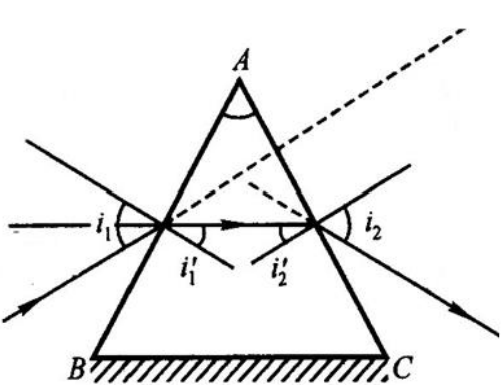
\includegraphics[width=0.3\textwidth]{tri.png}
    \caption{三棱镜折射示意图}
    \label{fig:tri}
\end{figure}
\\
根据几何关系,$A=i_1'+i_2'$;可以得到最小偏向角为:
\begin{align}
    \delta_{min}=2\arcsin(\frac{n_{\lambda}}{n_0}\sin(A/2))-A
\end{align}
\subsection{三棱镜的顶角}
三棱镜的顶角A在制造过程中可能存在误差,与制造标定的数值存在差异,因此我们采用反射法测定顶角:\\
首先将平行光管对准三棱镜顶角,光路如图所示:
\begin{figure}[h]
    \centering
    
\includegraphics[width=0.3\textwidth]{A.png}
    \caption{顶角测量示意图}
    \label{fig:A}
\end{figure}
\\
然后转动望远镜,分别观察到从两表面反射产生的狭缝像,对两游标作适当标记,两次分别记录两个游标游标1和游标2的读数。进而求出载物台转过的角度:\\
\begin{align}
    \Phi=\frac{1}{2}[|\theta_1-\theta_1'|+|\theta_2-\theta_2'|]
\end{align}
又由几何关系, $\Phi$是三棱镜顶角的两倍,故:
\begin{align}
    A=\Phi/2
\end{align}

\section{实验过程和数据分析}
\subsection{调整分光计}
调整分光计,需要达到下列要求:
\begin{enumerate}
    \item 平行光管发出平行光:
    \item 望远调整分光计,最后要达到下列要求:镜对平行光聚焦(即接收平行光)。
    \item 望远镜、平行光管的光轴垂直仪器公共轴
\end{enumerate}
分光计调整的关键是\textbf{调好望远镜},其他的调整可以以望远镜为基准。
\subsection{测量三棱镜顶角}
在这里我们使用原理中提到的反射法进行测量,多次测量取平均值,记录数据如下:
\\
\begin{table}[h]
    \begin{center}
        \begin{tabular}{|c|c|c|c|c|c|}
            \hline
           测量序号 & \(\theta_1\) & \(\theta_1'\) & \(\theta_2\) & \(\theta_2'\) & A \\
            \hline
           1 & \(108^\circ 7'\) & \(288^\circ 7'\) & \(228^\circ 10'\) & \(48^\circ 10'\) & \(60^\circ 1'30''\) \\
            \hline
           2 & \(94^\circ 20'\) & \(274^\circ 19'\) & \(214^\circ 21'\) & \(34^\circ 19'\) & \(60^\circ 0'30''\) \\
            \hline
          3 & \(115^\circ 23'\) & \(295^\circ 21'\) & \(235^\circ 25'\) & \(55^\circ 25'\) & \(60^\circ 3'\) \\
            \hline
        \end{tabular}
        \caption{三棱镜顶角测量数据}
        \label{table:1}
    \end{center}  
\end{table}

角度测量的不确定度为:
\begin{align}
    \delta_{Aa} &=\sqrt{\frac{\Sigma_i (A_i-A)^2}{n(n-1)}}=43'' \\ \delta_{Ab}&=\frac{1'}{\sqrt3}=34'' \\ \delta_A&=\sqrt{\delta_{Aa}^2+\delta_{Ab}^2}=55''\approx 1'
\end{align}
故测得顶角为:
\[A=60^\circ 1' \pm 1' \]
\subsection{测量三棱镜的色散曲线}
使用汞灯作为光源,用上文所述的最小偏向角法测量汞灯各谱线在玻璃中的折射率;\\
汞灯的发光谱线如下:\\
\begin{table}[h]
    \begin{center}
        \begin{tabular}{|c|c|c|c|c|c|c|c|c|}  
            \hline    
            波长(nm)& 404.66 & 435.84 & 496.16 & 546.07 & 576.96 & 578.97 & 623.44 & 690.72 \\
            \hline
            颜色 & 紫 & 蓝紫  & 青 & 绿 & 黄 & 黄 & 红 & 深红 \\
            \hline
            强度 &强 &很强 & 强 &很强 & 强 & 强 & 中 & 弱 \\
            \hline
        \end{tabular}
        \caption{汞灯发光谱线}
    \end{center}
\end{table}
\\
由于汞灯亮度和实验器材所限,肉眼仅能观察到404nm,435nm,496nm,546nm,576nm五条谱线。
\\
以下是它们在三棱镜中的最小偏向角数据:\\
\begin{table}[h]
    \begin{center}
        \begin{tabular}{|c|c|c|c|c|c|}
        \hline
        \(\lambda \ (nm)\)&404.66 & 435.84 & 496.16 & 546.07 & 576.96 \\
        \hline
        \(\theta\)&320°12'&320°30'&320°53'&321°13'&321°20'\\
        \hline
        \(\theta'\)&140°12'&140°30'&140°52'&141°11'&141°18'\\
        \hline
        \(\delta\)&39°48'&39°30'&39°07'&38°45'&38°41'\\
        \hline
        \end{tabular}
        \caption{汞灯谱线最小偏向角数据}
    \end{center}
\end{table}\\
其中,546nm的谱线进行了三次测量,数据记录如下:\\
\begin{table}[h]
    \begin{center}
        \begin{tabular}{|c|c|c|c|}
            \hline
            测量序号 & \(\theta\) & \(\theta'\) & \(\delta_i\)\\
            \hline
            1 & 320°53' & 140°52' & 39°7'30'' \\
            \hline
            2 & 321°14' & 141°13' & 38°46'30'' \\
            \hline
            3 & 321°14' & 141°13' & 38°46'30'' \\
            \hline
        \end{tabular}
        \caption{546nm谱线最小偏向角多次测量数据}
    \end{center}
\end{table}
\subsubsection{计算折射率}
根据公式(4)和(5)计算得到的所有谱线折射率数据如下:\\
\begin{table}[h]
    \begin{center}
        \begin{tabular}{|c|c|c|c|c|c|}
            \hline
            波长(nm)& 404.66 & 435.84 & 496.16 & 546.07 & 576.96 \\
            \hline
            折射率 & 1.5300 & 1.5266 & 1.5223 & 1.5181 & 1.5174 \\
            \hline
        \end{tabular}
        \caption{汞灯谱线折射率数据}
    \end{center}
\end{table}
\\
计算得到的546nm谱线折射率数据如下:\\
\begin{align}
    n_\lambda=\frac{n_0}{\sin(A/2)}\sin(\frac{\delta_{min}+A}{2})=1.5223
\end{align}
计算不确定度:
\begin{align}
    u_\delta&=\sqrt{u_{\delta_a}^2+u_{\delta_b}^2}=\sqrt{\frac{\Sigma_1^3(\delta_i-\bar{\delta})^2}{6}+\frac{1'^2}{3}} \\
    u_{n}&=\sqrt{(\frac{\partial n_{\lambda}}{\partial A} u_A)^2+(\frac{\partial n_{\lambda}}{\partial \delta_{\lambda}^{min}}u_{\delta})^2}
\end{align}
得到最终实验结果:
\begin{align}
    n_{546nm}=1.5197\pm 0.0003
\end{align}
\\
\subsubsection{绘制色散曲线、拟合Cauchy方程}
根据表绘制色散曲线,并使用拟合方法拟合Cauchy方程,得到拟合结果如下:
\\
\begin{figure}[h]
    \centering
    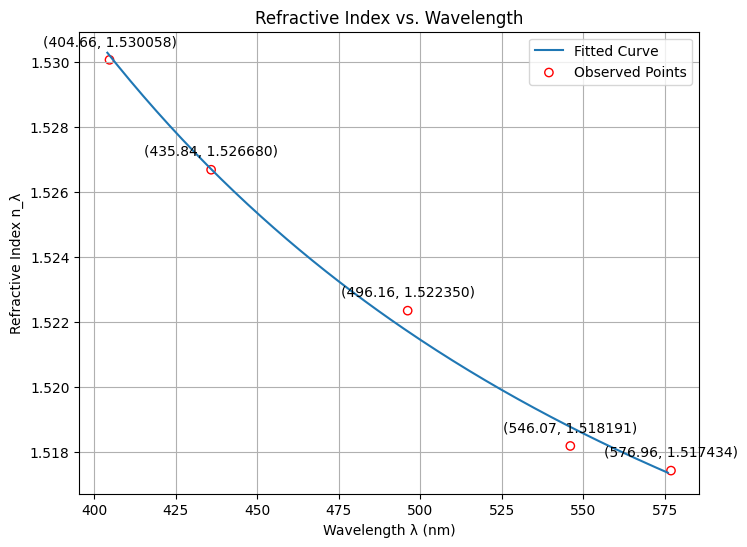
\includegraphics[width=0.8\textwidth]{fit.png}
    \caption{\(n_\lambda - \lambda\)关系(拟合)}
    \label{fig:fit}
\end{figure}
\\
其中拟合结果如下所示:
\begin{center}
    A=1.504870 (nm), B=4146.749084 (\(nm^2\)), C=1.000000 (\(nm^4\))
\end{center}
拟合所用程序见附录。
\section{分析与讨论}

\subsection{误差分析}

\subsubsection{实验中的系统误差}
来自xxx的精度影响。

受空间内xx与xx的干扰。

\subsubsection{实验中的偶然误差}
接线时可能有xxx情况,导致xxx。xx上的xx在某情况下有xx的问题存在,经反复调整后得以正常测量。

\subsection{实验后的思考}
可说明自己做本实验的总结、收获和体会,对实验中发现的问题提出自己的建议。

\newpage
%图一般很大,建议换页。
\section{附录}
\begin{python}
    
    import pandas as pd
    import re
    import math
    import matplotlib.pyplot as plt
    from scipy.optimize import curve_fit

    def dms_to_radians(dms_str):
        parts = re.split(r'[°\'\"]', dms_str)
        degrees = int(parts[0])
        minutes = int(parts[1]) if len(parts) > 1 and parts[1] else 0
        seconds = int(parts[2]) if len(parts) > 2 and parts[2] else 0
    
        decimal_degrees = degrees + minutes / 60 + seconds / 3600
        radians = math.radians(decimal_degrees)
        return radians

    df = pd.read_csv('data.csv')
    df['n_lambda'] = n_0 / math.sin(A_rad / 2) * df['delta(rad)'].apply(lambda x: math.sin((x + A_rad) / 2))

    def dispersion_equation(wavelength, A, B, C):
        return A + B / wavelength**2 + C / wavelength**4

    popt, _ = curve_fit(dispersion_equation, df['lambda(nm)'], df['n_lambda'])

    A, B, C = popt

    wavelength_range = pd.Series(range(int(df['lambda(nm)'].min()), int(df['lambda(nm)'].max()) + 1))
    fitted_n = dispersion_equation(wavelength_range, A, B, C)

    plt.figure(figsize=(8, 6))
    plt.plot(wavelength_range, fitted_n, label='Fitted Curve')
    plt.scatter(df['lambda(nm)'], df['n_lambda'], color='red', marker='o', facecolors='none', label='Observed Points')

    for i, row in df.iterrows():
        plt.annotate(f"({row['lambda (nm)']}, {row['n_lambda']:.6f})", (row['lambda (nm)'], row['n_lambda']), textcoords="offset points", xytext=(0, 10), ha='center')

    plt.xlabel('Wavelength lambda (nm)') 
    plt.ylabel('Refractive Index n_lambda')
    plt.title('Refractive Index vs. Wavelength')
    plt.legend()
    plt.grid(True)
    plt.show()

    print(f"Fitted Parameters: A={A:.6f}, B={B:.6f}, C={C:.6f}")
    
\end{python}
\bibliographystyle{plain}
\bibliography{./template}  %bib文件名

\end{document}
